%\documentclass[a4paper]{scrartcl}
\documentclass[a4paper]{article} \usepackage{setspace}
\usepackage{url}
\usepackage{mdwlist}
\usepackage{polski}
\usepackage[utf8x]{inputenc}
\usepackage{color}
\usepackage{mathtools}
\usepackage{graphicx}
\usepackage[unicode=true]{hyperref}
\usepackage{multirow}
\usepackage[table]{xcolor}
\usepackage{subfig}
\usepackage{listings}
\usepackage[backgroundcolor=white]{todonotes}
\definecolor{dkgreen}{rgb}{0.2,0.8,0.2}
\definecolor{gray}{rgb}{0.5,0.5,0.5}
\definecolor{mauve}{rgb}{0.58,0,0.82}
\newcommand{\HRule}{\rule{\linewidth}{0.5mm}}
\newcommand{\siatkonator}{\textbf{Siatkonator} }
\renewcommand{\triangle}{\href{http://www.cs.cmu.edu/~quake/triangle.html}{triangle}}
\lstset{ %
  basicstyle=\ttfamily\footnotesize,
  numbers=left,
  numberstyle=\footnotesize,
  stepnumber=1,
  numbersep=5pt,
  breaklines=true,
  tabsize=2,
  showspaces=false,
  showstringspaces=false,
  frame=single,
  numberstyle=\tiny\color{gray},
  keywordstyle=\color{mauve},
  commentstyle=\color{dkgreen},
  stringstyle=\color{mauve},
}

\begin{document}
\begin{titlepage}

  \begin{center}


    % Upper part of the page
    
\includegraphics[width=0.3\textwidth]{logo.jpg}\\[1cm]

    \begin{onehalfspace}
      \textsc{\LARGE Wydział Elektryczny Politechniki Warszawskiej}\\[1.5cm]
    \end{onehalfspace}



    \textsc{Języki i~Metody Programowania II -- projekt 1}\\[0.5cm]

    % Title
    \HRule \\[0.4cm]
    {\huge \bfseries Siatkonator }\\[0.2cm]
    \HRule \\[1.5cm]

    % Author and supervisor
    \begin{flushleft} \large
      \emph{Autor:}\\
      Barnaba \textsc{Turek}\\
      \href{mailto:barnabaturek@gmail.com}{barnabaturek@gmail.com}
    \end{flushleft}
    \vfill

    % Bottom of the page
    {\large \today}

  \end{center}

\end{titlepage}
\sloppy

\setcounter{tocdepth}{4}
\tableofcontents

\section{Specyfikacja funkcjonalna}
\subsection{Program}
\siatkonator to program sklejający siatki trójkątne.
Program przyjmuje jedną lub więcej siatek trójkątnych oraz jeden wielokąt.

Wynikiem działania programu jest siatka trójkątna opisująca zadany wielokąt, która zawiera podane określone siatki.

\begin{figure}[h]
  \centering
  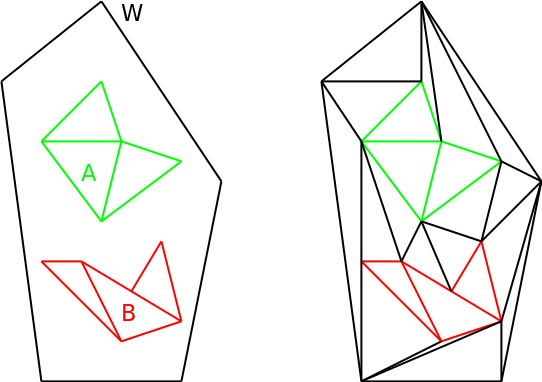
\includegraphics[width=0.5\textwidth]{ilustracja.png}
  \caption{przykład sklejania zadanego wielokątu W~i~siatek A~i~B}
\end{figure}

\subsection{Wywołanie}
Program nie prowadzi dialogu z~użytkownikiem.

\begin{lstlisting}[caption=Przykładowe wywołanie]
  $ siatkonator -e siatka1.ele -e siatka2.ele polygon.poly
\end{lstlisting}

Ostatni argument programu określa nazwę pliku (wraz ze ścieżką) w~którym opisany jest wielokąt.
Nie podanie tego argumentu spowoduje błąd wykonania programu.

Wcześniejsze argumenty określają opcje wykonania programu i~nie są wymagane.
Kolejność argumentów nie ma znaczenia.

Dostępne są następujące opcje:
\begin{description}
  \item[\texttt{-e <name>}] dodaje siatkę, która zostanie ``sklejona'' z~wielokątem. Program zakłada, że istnieje także plik o~takiej samej nazwie bazowej z~rozszerzeniem \texttt{node} opisujący wierzchołki.
  \item[\texttt{-o <name>}] podaje nazwę pliku wyjściowego. W~przypadku braku tego parametru wynik zostanie wypisany na standardowe wejście (najpierw plik ele, potem node).
  \item[\texttt{-q <angle>}] określa minimalny kąt w~dowolnym trójkącie wygenerowanej siatki (nie zmienia siatek wklejanych).
  \item[\texttt{-a <area>}] określa maksymalną powierzchnie dowolnego trójkąta w~generowanej siatce (j.w.).
  \item[\texttt{-d <eps>}] określa epsilon używany do porównywania koordynatów punktów w~celu stwierdzenia, czy należy je połączyć w~jeden punkt. Domyślnie program przyjmuje 0.005.
\end{description}

W~przypadku powodzenia program zwraca zero. W~przeciwnym wypadku program zwraca jeden z~kodów błędu:

\begin{description}
  \item[\texttt{kod 1}] Błąd otwarcia pliku (spowodowany np. brakiem uprawnień lub pliku).
  \item[\texttt{kod 2}] Błąd wczytania pliku (spowodowany błędnym formatem któregoś z~plików źródłowych).
  \item[\texttt{kod 3}] Błędny format argumentów linii poleceń.
\end{description}

Ponadto program w~czasie działania wypisuje informacje o~swoim aktualnym stanie na wyjście \texttt{STDERR}.

\subsection{Pliki}
\siatkonator korzysta z~plików w~formatach \texttt{poly}, \texttt{ele} i~\texttt{node}.

\begin{description}
  \item[poly] \href{http://www.cs.cmu.edu/~quake/triangle.poly.html}{format pliku opisującego wielokąt}
  \item[ele] \href{http://www.cs.cmu.edu/~quake/triangle.ele.html}{format pliku opisującego z~których wierzchołków składają się trójkąty siatki}
  \item[poly] \href{http://www.cs.cmu.edu/~quake/triangle.poly.html}{format pliku opisującego wierzchołki siatki}
\end{description}

Wszystkie wykorzystywane formaty są zgodne z~formatami wykorzystywanymi przez program \triangle.

\subsection{Obsługa atrybutów}
Atrybuty są zachowywane.
Wymagane jest, aby wszystkie pliki wejściowe miały taką samą liczbę atrybutów.

W~przypadku połączenia dwóch wierzchołków, zostaną zachowane atrybuty jednego z~nich.

\subsection{Rozwiązywanie konfliktów znaczników wierzchołków}
Wczytując pliki program zapamiętuje najniższy i~najwyższy znacznik wierzchołka w~danym pliku.
Następnie program oblicza stałą, o~którą należy przesunąć znacznik wierzchołka w~tym pliku, aby nuniknąć konfliktu.

\begin{lstlisting}[caption=Przykład]
  Jezeli w~pliku A.poly znaczniki wierzcholkow sa z~zakresu 1..10,
  I~w~pliku B.node znaczniki sa z~zakresu 3..10,
  I~po wczytaniu B.node najwiekszy znaleziony znacznik bedzie 10,
  To po wczytaniu A.poly najmniejszy znaleziony znacznik jest 3,
  Wiec nalezy wszystkie znaczniki wierzcholkow znalezionych w~A.poly przesunac o~(10-3)
\end{lstlisting}

W~związku z~tym wynik działania programu \textbf{zależy} od kolejności podanych plików wejściowych
(Z~tym ze znaczniki z~otoczki zawsze maja najwyższe wartości).

Po takim podziale pozostała przestrzeń zmiennej używana jest do rozwiązywania konfliktów wynikających z~tego, że dwa wierzchołki o~różnych znacznikach znalazły się w~tym samym miejscu.

Jeśli oba wierzchołki zajmujące te same koordynaty mają różną wartość znaczników, zostaje im przydzielona nowa wartość z~zakresu wartości przeznaczonego na konflikty za pomocą prostej funkcji mieszającej

\begin{lstlisting}[caption=]
(znacznik\ A + znacznik\ B) % (wolne miejsce w~zakresie INTa) + offset zakresu
\end{lstlisting}

Takie rozwiązanie gwarantuje, że elementy będące połączeniem danych znaczników zawsze będą miały ten sam znacznikw~pliku wynikowym.

\begin{figure}[h]
  \centering
  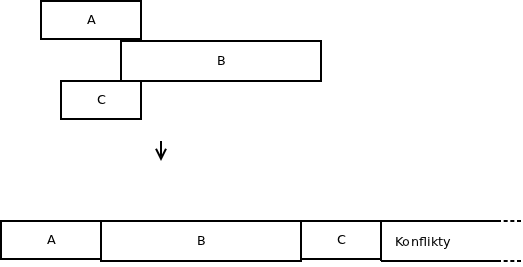
\includegraphics[width=0.8\textwidth]{konflikty.png}
  \caption{przykład podziału przestrzeni znaczników}
\end{figure}
\newpage
\subsection{Instalacja}
Program nie wymaga instalacji.
\subsection{Kompilacja}
Program można skompilować korzystając z~programu \texttt{GNU make}.
Proces kompilacji jak i~sam program był testowany na systemie Linux.

Program ma jedną zależność, bibliotekę \emph{argtable2}.

Aby uniknąć instalowania pakietu argtable-dev z~repozytorium dystrybucji, dołączyłem go do repozytorium SVN.
Wywołanie polecenia \texttt{make} powinno zbudować tę zależność, jednak kompilacja wymaga programu \texttt{cmake}.

\section{Specyfikacja implementacyjna}
\subsection{Struktura programu}

\begin{figure}[h]
  \centering
  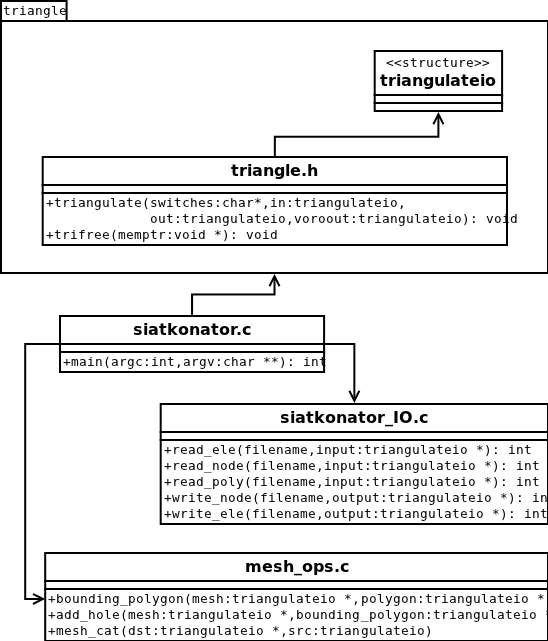
\includegraphics[width=0.8\textwidth]{class.png}
  \caption{Diagram klas}
\end{figure}

  Program podzielony jest na następujące moduły:
  \begin{description}
    \item[siatkonator.c] Plik zawierający główną funkcję odpowiedzialną za wczytanie argumentów i~zależnie od nich wykonanie algorytmu sklejania siatek.
    \item[siatkonator\_IO] Katalog (moduł) zawierający funkcje związane z~czytaniem i~zapisywaniem plików \emph{node}, \emph{ele} i \emph{poly} do struktur \texttt{triangulateio}.
    \item[mesh\_ops.c] Plik zawierający funkcje obsługujące logikę sklejania siatek (znajdowanie wielokąta otaczającego siatkę, wycinanie dziur w~siatkach i~łączenie siatek).
    \item[common.c] Plik zawierający funkcje pomocnicze (takie jak wypisywanie wiadomości). \texttt{common.h} zawiera także struktury używane do przekazywania danych wewnątrz programu.
    \item[markers.c] Plik zawierający funkcje służące przesuwaniu i~rozwiązywaniu konfliktów znaczników.
    \item[siatkonator\_hash.c] Plik zawierający funkcje i~strukturę danych obsługującą tablicę mieszającą używaną do znajdowania wielokąta otaczającego siatkę..
  \end{description}

\subsubsection{Funkcje modułu \texttt{mesh\_ops}}
\begin{description}
  \item[\texttt{bounding\_polygon}] funkcja przyjmująca wskaźnik na wczytaną siatkę i~znajdująca otaczający ją wielokąt (który należy wyciąć z~otoczki przed przeprowadzeniem triangulacji).
  \item[\texttt{bounding\_polygon\_hole}] funkcja dodająca do otoczki dziurę o~współrzędnych równych środkowi ciężkości pierwszego trójkąta z~dodawanej siatki.
  \item[\texttt{add\_bounds\_as\_segments}] funkcja dodająca znaleziony wcześniej otaczający wielokąt do otoczki.
  \item[\texttt{mesh\_cat}] Funkcja przyjmująca dwa wskaźniki na siatki i~dodająca elementy drugiej siatki do elementów pierwszej siatki.
  \item[\texttt{remove\_duplicates}] Funkcja usuwająca wierzchołki o~identycznych lub podobnych współrzędnych.
\end{description}

\subsection{Algorytmy}
\begin{lstlisting}[caption=Pseudokod algorytmu głównej funkcji programu sklejającej siatki]
  wczytaj dane z pliku poly do struktury p
  dla kazdego pliku .ele:
    wczytaj dane z plikow ele i nodes do struktury E
    znajdz w strukturze E krawedzie, ktore wystepuja tylko raz
    dodaj te krawedzie do struktury P jako sekcje
    dodaj dziure do struktury P wewnatrz pierwszego trojkata ze struktury E
  wykonaj triangulacje na strukturze p do siatki S
  dla kazdego pliku .ele:
    wstaw siatke z pliku do dziur w siatce S
  usun powtarzajace sie wierzcholki
  zapisz wynik triangulacji do plikow ele i node
\end{lstlisting}

\begin{lstlisting}[caption=Pseudokod funkcji szukającej wielokąta otaczającego daną siatkę: \texttt{bounding\_polygon}]
  H - tablica mieszajaca

  Dla kazdego wierzcholka w:
    jezeli H[w] istnieje:
      Dodaj w do H
    else:
      Usun w z~H

  Dla kazdego wierzcholka w:
    jezeli H[w] istnieje:
      dodaj w~do wielokata otaczajacego
      usun w~z~wielokata otaczajacego

  Dodaj dziure w~wielokacie otaczajacym w~miejscu srodka ciezkosci pierwszego elemenetu.

\end{lstlisting}

\subsection{struktury danych}
Struktura danych używana do komunikacji między funkcjami to struktura \texttt{triangulateio} dostarczona wraz z~programem triangle.
Struktura ta pozwala opisać siatkę na każdym etapie jej budowania (także siatki wyjściowe).

Jej wadą jest fakt, że nie jest specjalizowana do konkretnych zadań i~wiele pól nie będzie miało zastosowania.
Mimo to jest już napisana, udokumentowana i~mogę być pewien, że zawiera wszystkie potrzebne pola.

Zastosowanie innej struktury, jako struktury pośredniej wymagałoby tłumaczenia jej do \texttt{triangulateio} przed wykonaniem funkcji \texttt{triangulate()}.

Zastosowana jest także tablica mieszająca, w~której konflikty rozwiązywane są za pomocą listy.
Tablica potrafi też zwrócić wszystkie swoje elementy w~formie listy.


\section{Testy aplikacji}
\subsection{Testy automatyczne}
Aplikacja zawiera kilkanaście testów automatycznych napisanych na początku w~języku Ruby.
Testy te sprawdzają rzeczy łatwe do sprawdzenia z~zewnątrz - obsługę argumentów, poprawność wczytywania plików.
Przy okazji testy były bardzo pomocne jako wczesny wskaźnik tego, że coś się zepsuło - bardzo podstawowe testy regresyjne, polegające na uruchomieniu programu i~sprawdzeniu jego kodu wyjścia.

Zostały zaimplementowane następujące testy:
\begin{lstlisting}[caption=Testy automatyczne]
siatkonator IO
  when it reads square.poly
    should read poly file without error
    should read nodes coordinates and attributes properly
    should read nodes segments and holes properly
  when it reads square-firstnode-1.poly
    should read poly file without error
    should read nodes coordinates and attributes properly
    should read nodes segments and holes properly
  when it reads square-firstnode-1.poly
    should read poly and ele files without error
    should read 1.ele and 1.node properly
    should read 2.ele and 2.node properly

siatkonator argument reader
  should require at least one option
  should be ok when option given
  should fail when the only option is preceded with switch
  should notify that max surface was set
  should notify that min angle was set
  should notify that mesh files were provided
  should notify that output file was set

Finished in 0.09719 seconds
16 examples, 0 failures

\end{lstlisting}

\subsection{Tryb debug}
Aplikacja wyposażona jest w tryb wspomagający testowanie, w którym wypisuje swój stan na standardowe wyjście.
To, czy aplikacja działa w tym trybie zależy od flag kompilacji.

Ponieważ nie chciałem uzależniać moich funkcji od zmiennych globalnych i wypisywania danych (ze względu na \emph{Single Responsibility Principle}) ograniczyłem całe wypisywanie do funkcji siatkonator log,
która w~razie czego może zostać zastąpiona pustą funkcją. Zbieranie informacji diagnostycznych w~funkcji main byłoby bardzo kłopotliwe i~spowodowałoby, że funkcja rozrosłaby się jeszcze bardziej.

Aplikacja wypisuje zawartość struktur \texttt{triangulateio} na następujących etapach:
\begin{itemize}
  \item wczytanie plików (poly, node+ele);
  \item znalezienie wielokąta ograniczającego;
  \item dodanie wielokąta ograniczającego i~dziury;
  \item po/przed wywołaniu funkcji triangulate;
  \item po ponownym dodaniu siatek
  \item po usunięciu duplikatów
\end{itemize}

Ponadto program wypisuje różne informacje podsumowujące jego działanie, takie jak np. informacja z~jakich plików będzie korzystał i~ile wierzchołków wczytał.

\subsection{Testy eksploracyjne}
Testy, których większość była wykonywana w~czasie pisania programu polegające na sprawdzaniu, czy robi to co powinien robić.
Do tych testów stosowałem własne pliki, przykładowe pliki dostępne na stronie \texttt{wikidyd}, pliki testowe kolegi oraz plik przedstawiający literę 'A' będący częścią dystrybucji Triangle.

\newpage
\subsubsection{Podstawowe testy}
Pierwsze dwa proste testy, które przeprowadziłem dotyczyły kwadratowej otoczki.
Testy korzystały z~najprostszych możliwych siatek - trójkątów.
W~jednym teście wklejono do otoczki jedną siatkę, w~drugim dwie.

Komendy, za pomoca ktorych uzyskalem te wyniki sa nastepujace\footnote{wszystkie pliki z~których korzystałem do testów są w~repozytorium}:
\begin{lstlisting}
./bin/siatkonator -a 0.01 -e spec/data/2.ele -o test spec/data/square-no-holes.poly
./bin/siatkonator -a 0.001 -e spec/data/1.ele -e spec/data/2.ele -o test spec/data/square-no-holes.poly
\end{lstlisting}

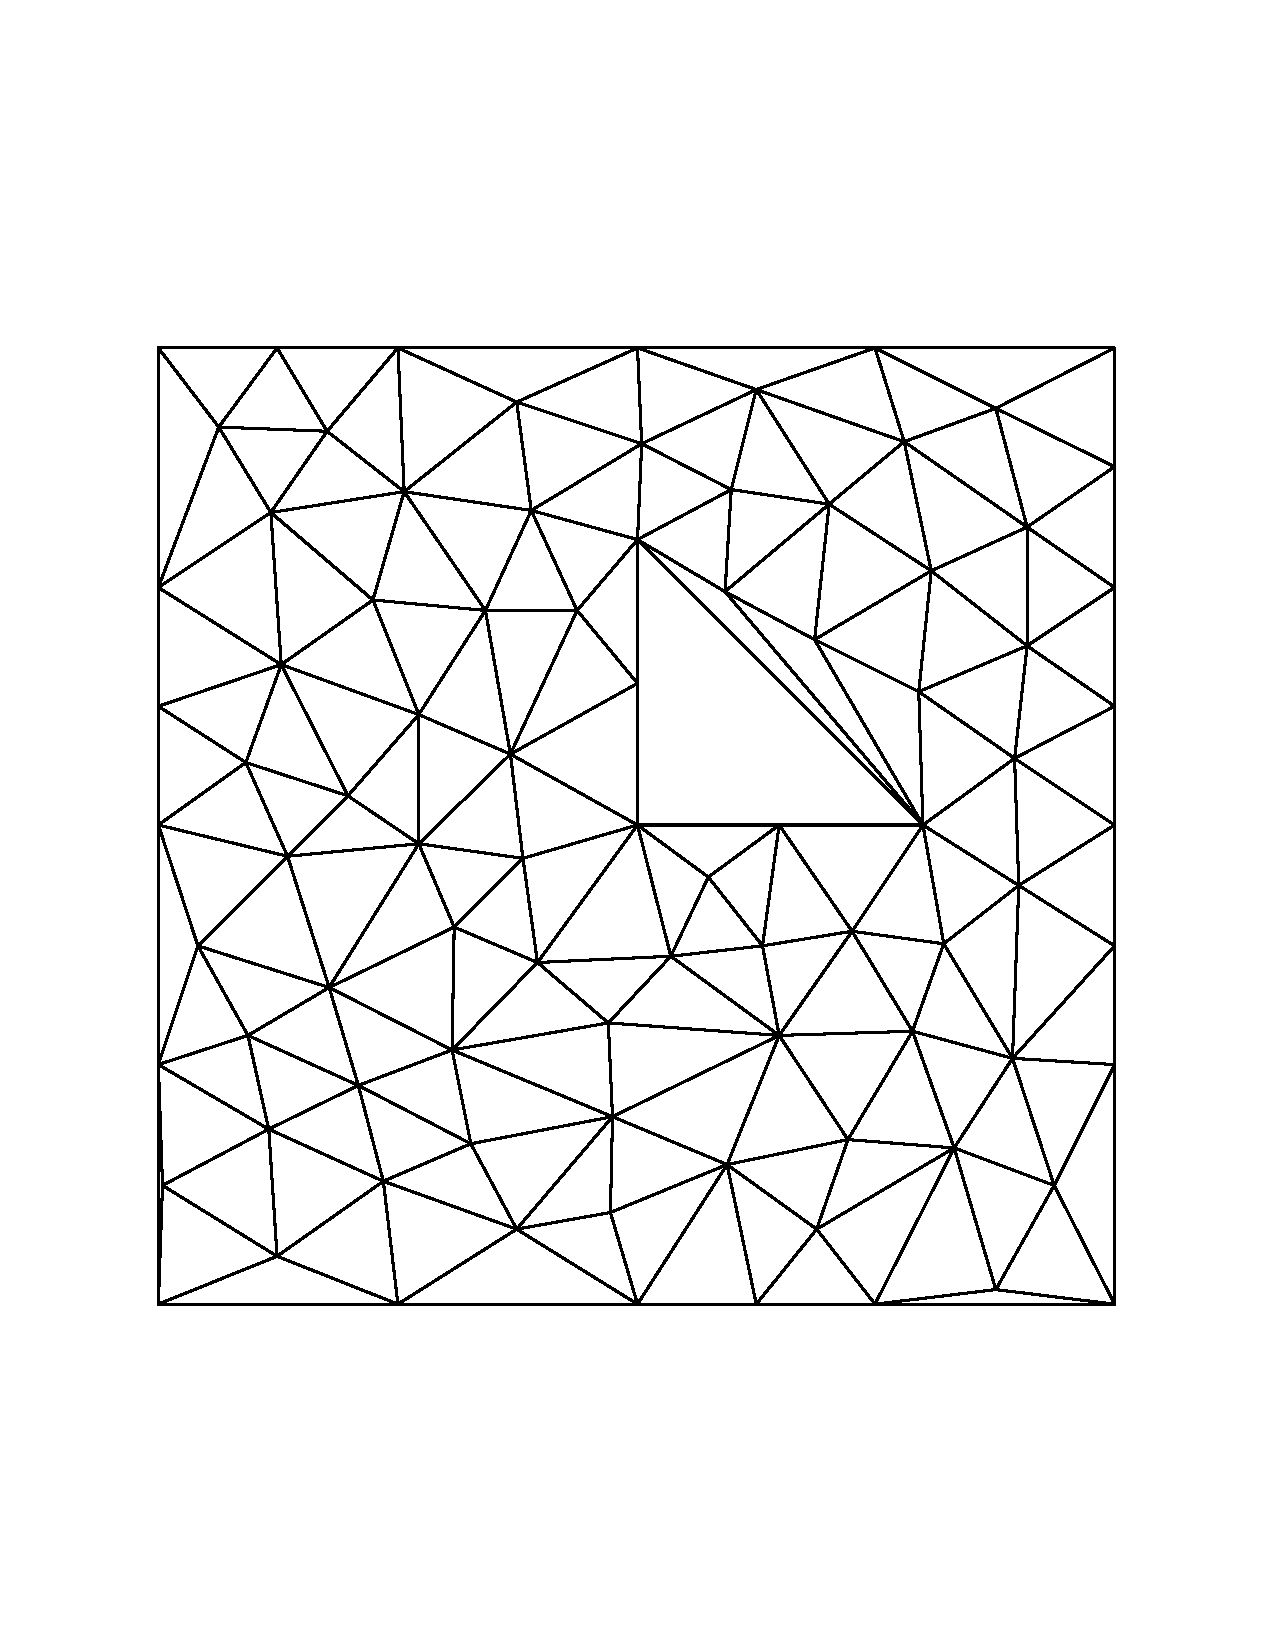
\includegraphics[width=0.5\textwidth]{1_trojkat.pdf}
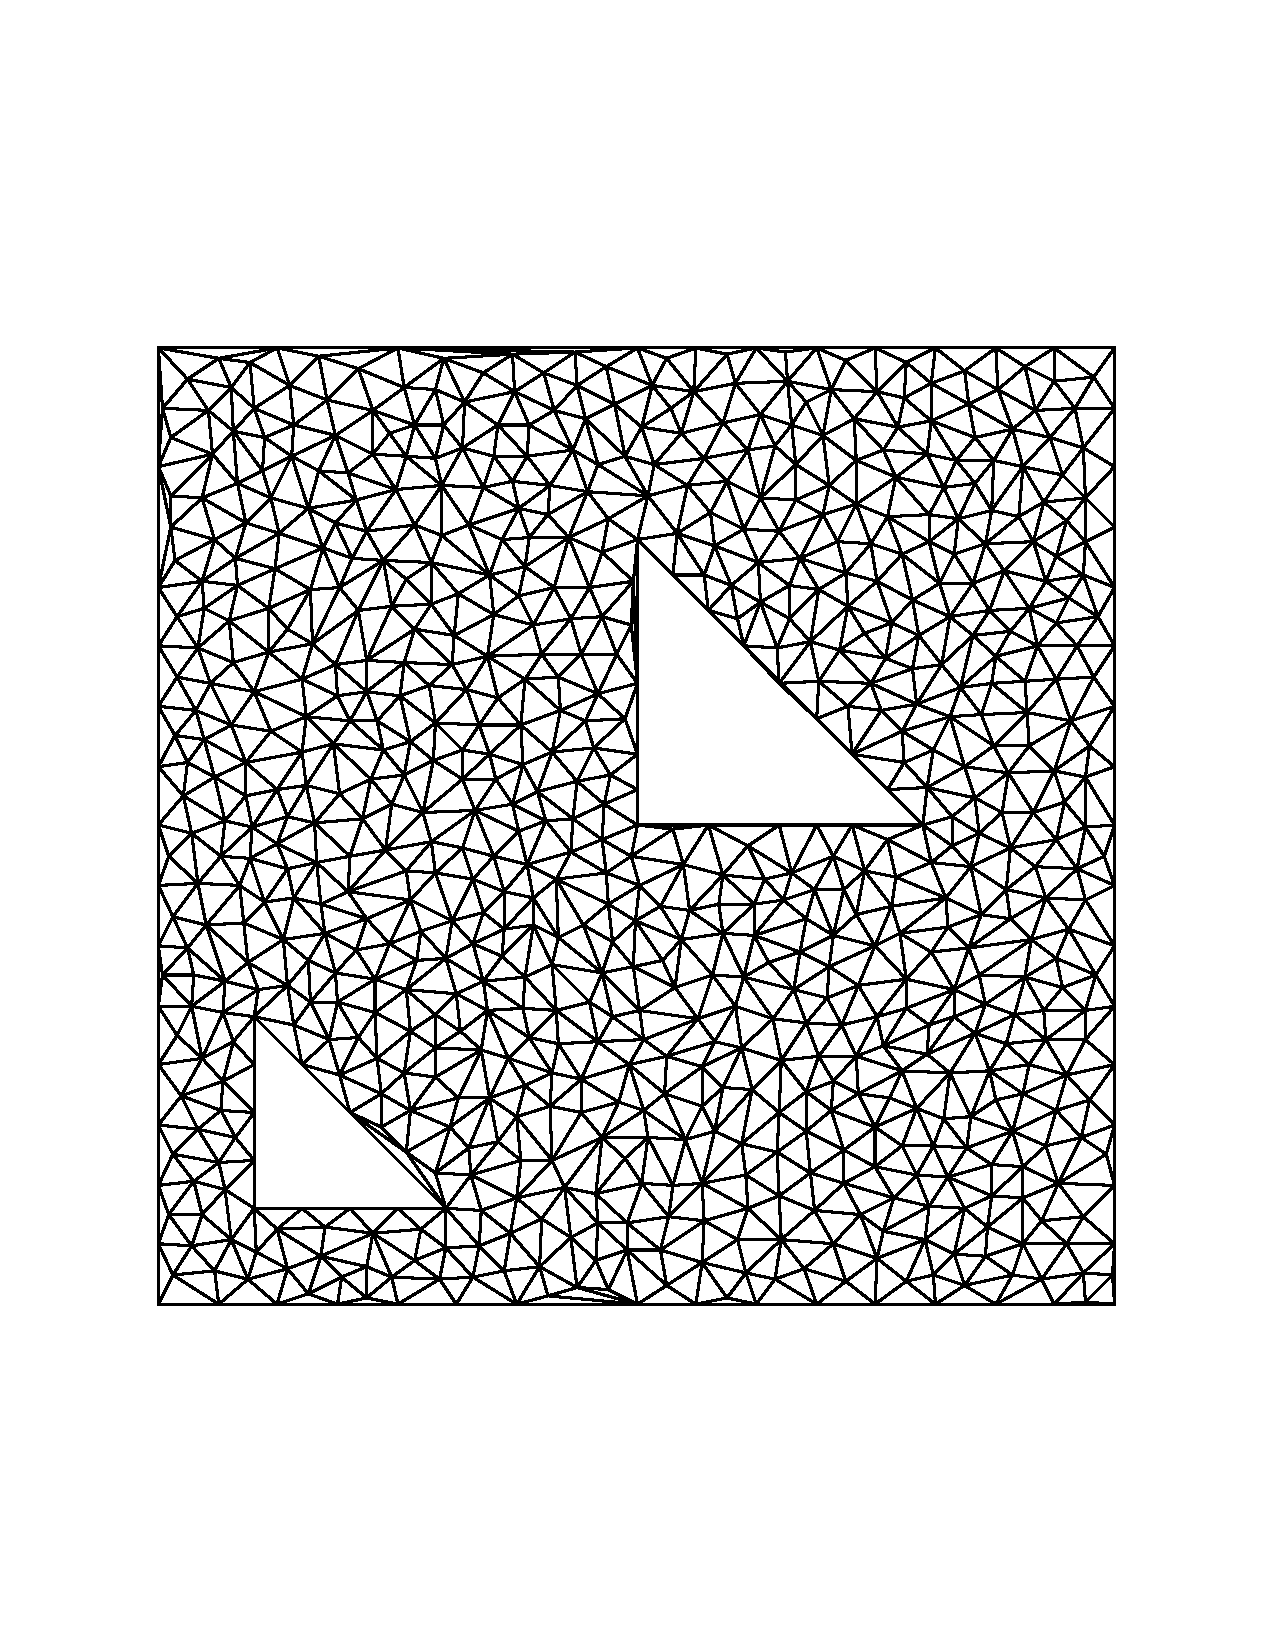
\includegraphics[width=0.5\textwidth]{2_trojkaty.pdf}

\subsubsection{Test wyznaczania otoczki}
W~następnym teście skorzystałem z~bardziej złożonej siatki - kwadratu złożonego z~trzech trójkątów.
Miało to na celu upewnienie się, że funkcje określające wielokąt otaczający działają zgodnie z~założeniami.

W~ramach tego testu wydałem dwa razy te samą komendę, ale za pierwszym razem wykomentowałem wywołanie funkcji wklejającej siatkę do przeznaczonej dla niej dziury:
\begin{lstlisting}
# wykomentowano 'mesh_cat(&out, meshes + i);'
./bin/siatkonator -a 0.001 -e spec/data/kwadrat.ele -o test spec/data/square-no-holes.poly
# odkomentowano
./bin/siatkonator -a 0.001 -e spec/data/kwadrat.ele -o test spec/data/square-no-holes.poly
\end{lstlisting}

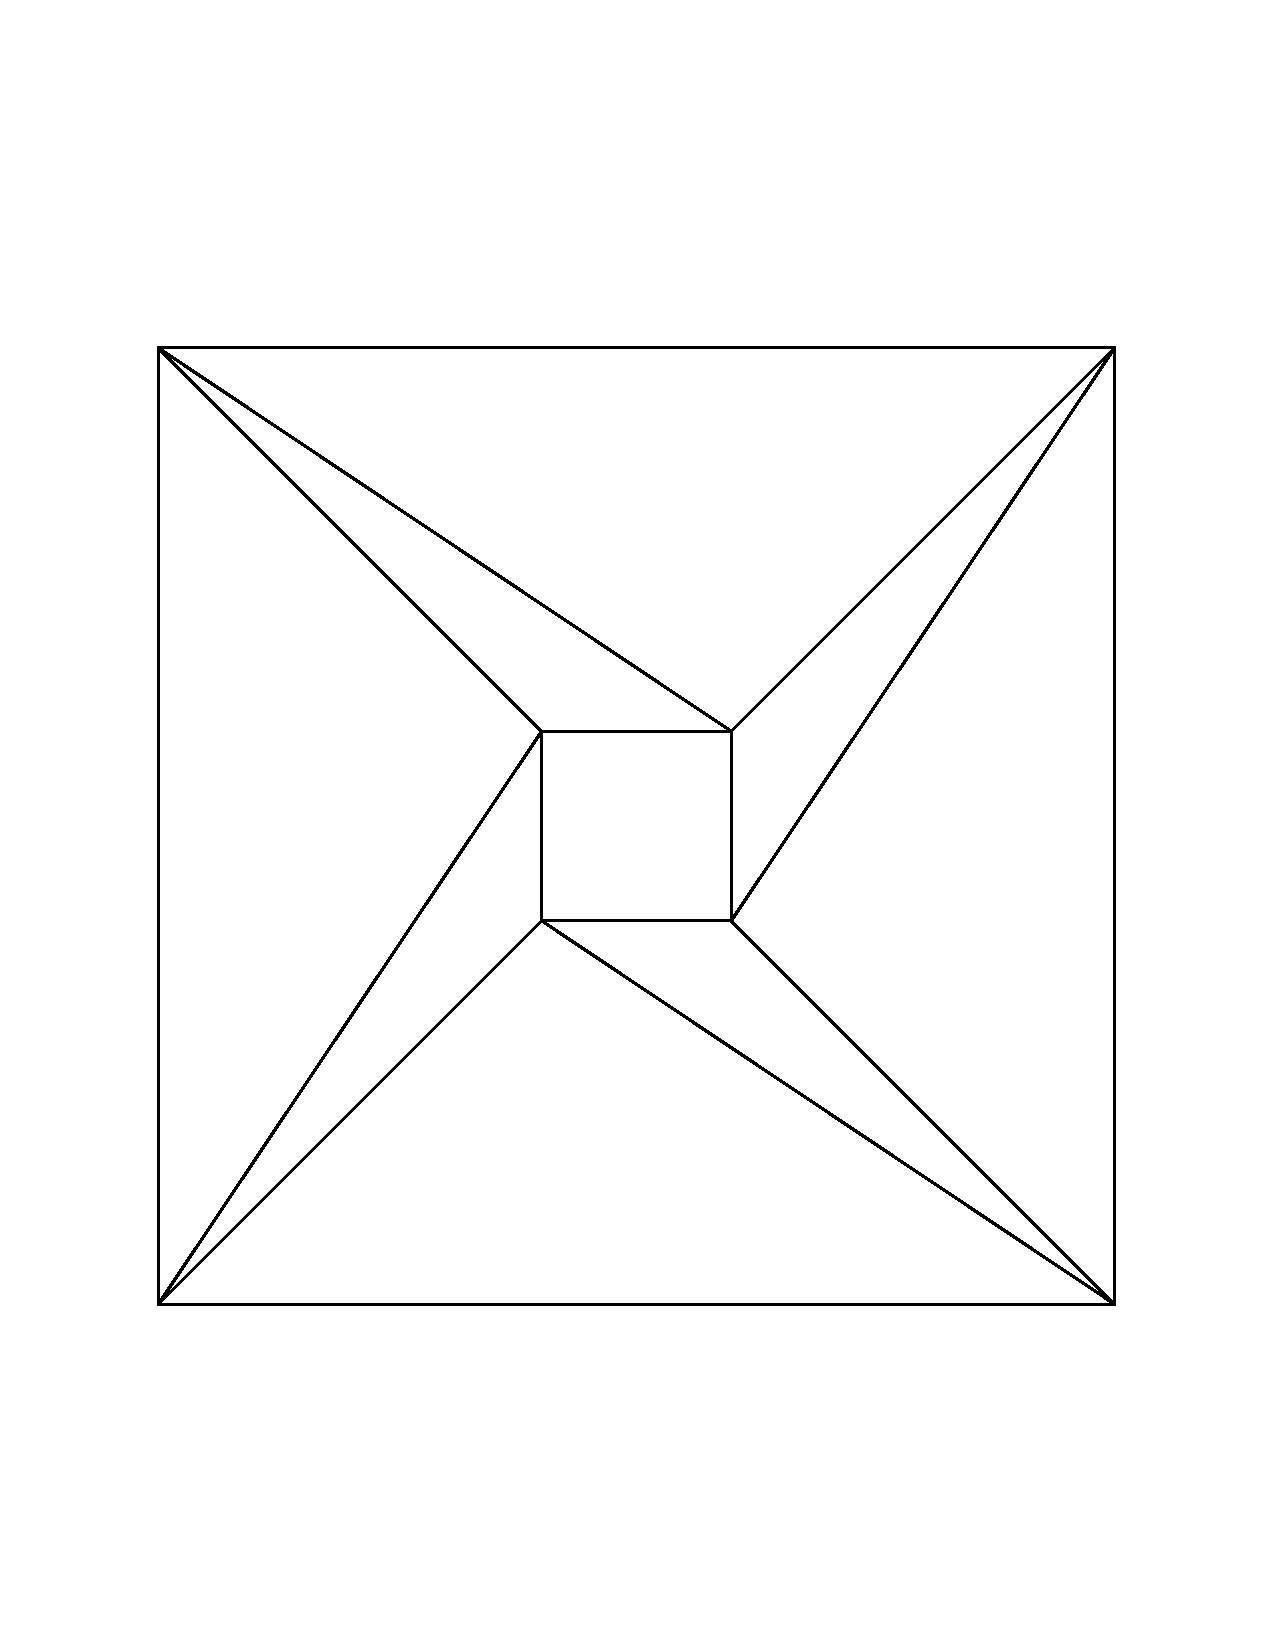
\includegraphics[width=0.5\textwidth]{kwadrat_empty.pdf}
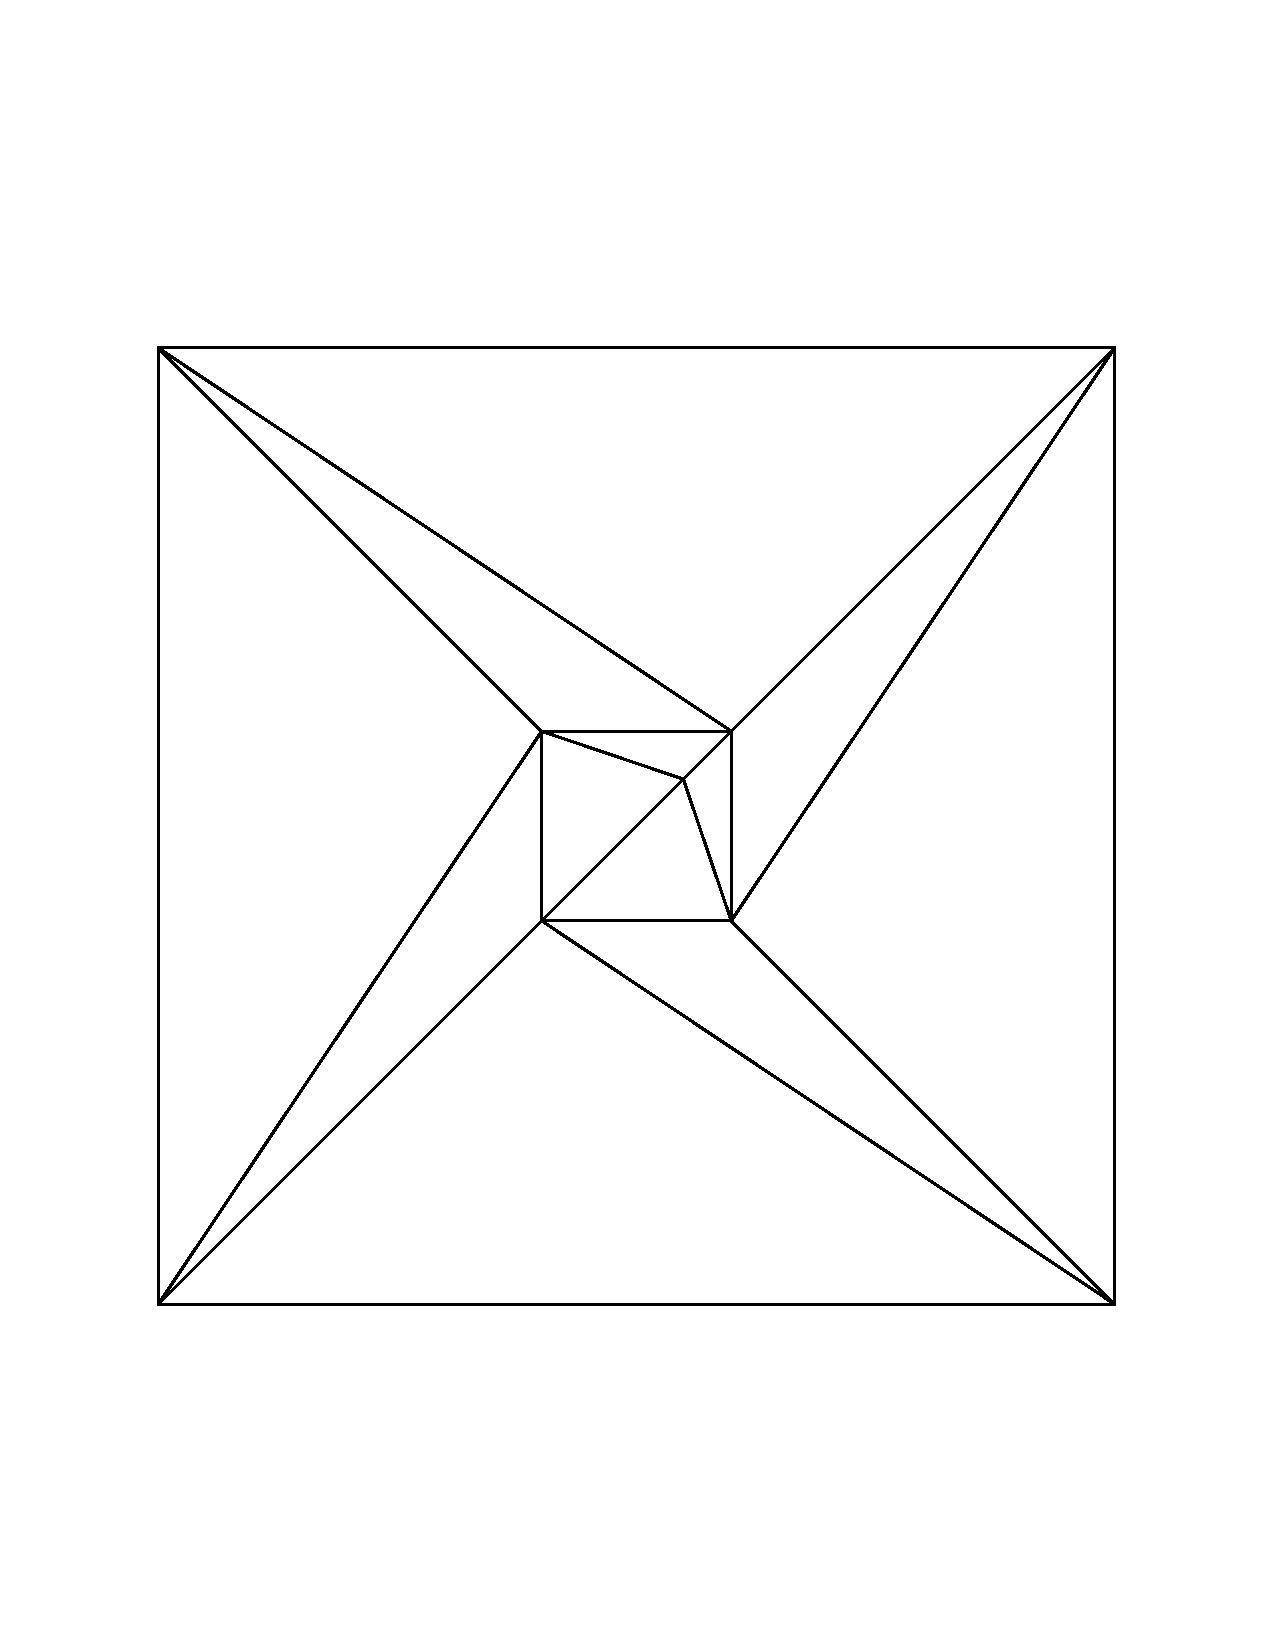
\includegraphics[width=0.5\textwidth]{kwadrat_full.pdf}

Dzięki temu zabiegowi można się przekonać, że wielokąt otaczający, w~tym wypadku kwadrat, został wyznaczony poprawnie oraz że zostały z~niego usunięte wszystkie wierzchołki i~segmenty, które nie są częścią wielokąta otaczającego.

\subsubsection{Element mechaniczny z~dziurką}
Test polegał na sklejeniu otoczki z~siatką, która zawierała dziurę.
jego celem jest sprawdzenie, czy dziura zostanie poprawnie wypełniona trójkątami.
\begin{lstlisting}
./bin/siatkonator -a 0.001 -e spec/data/kwadrat.ele -o test spec/data/square-no-holes.poly
\end{lstlisting}
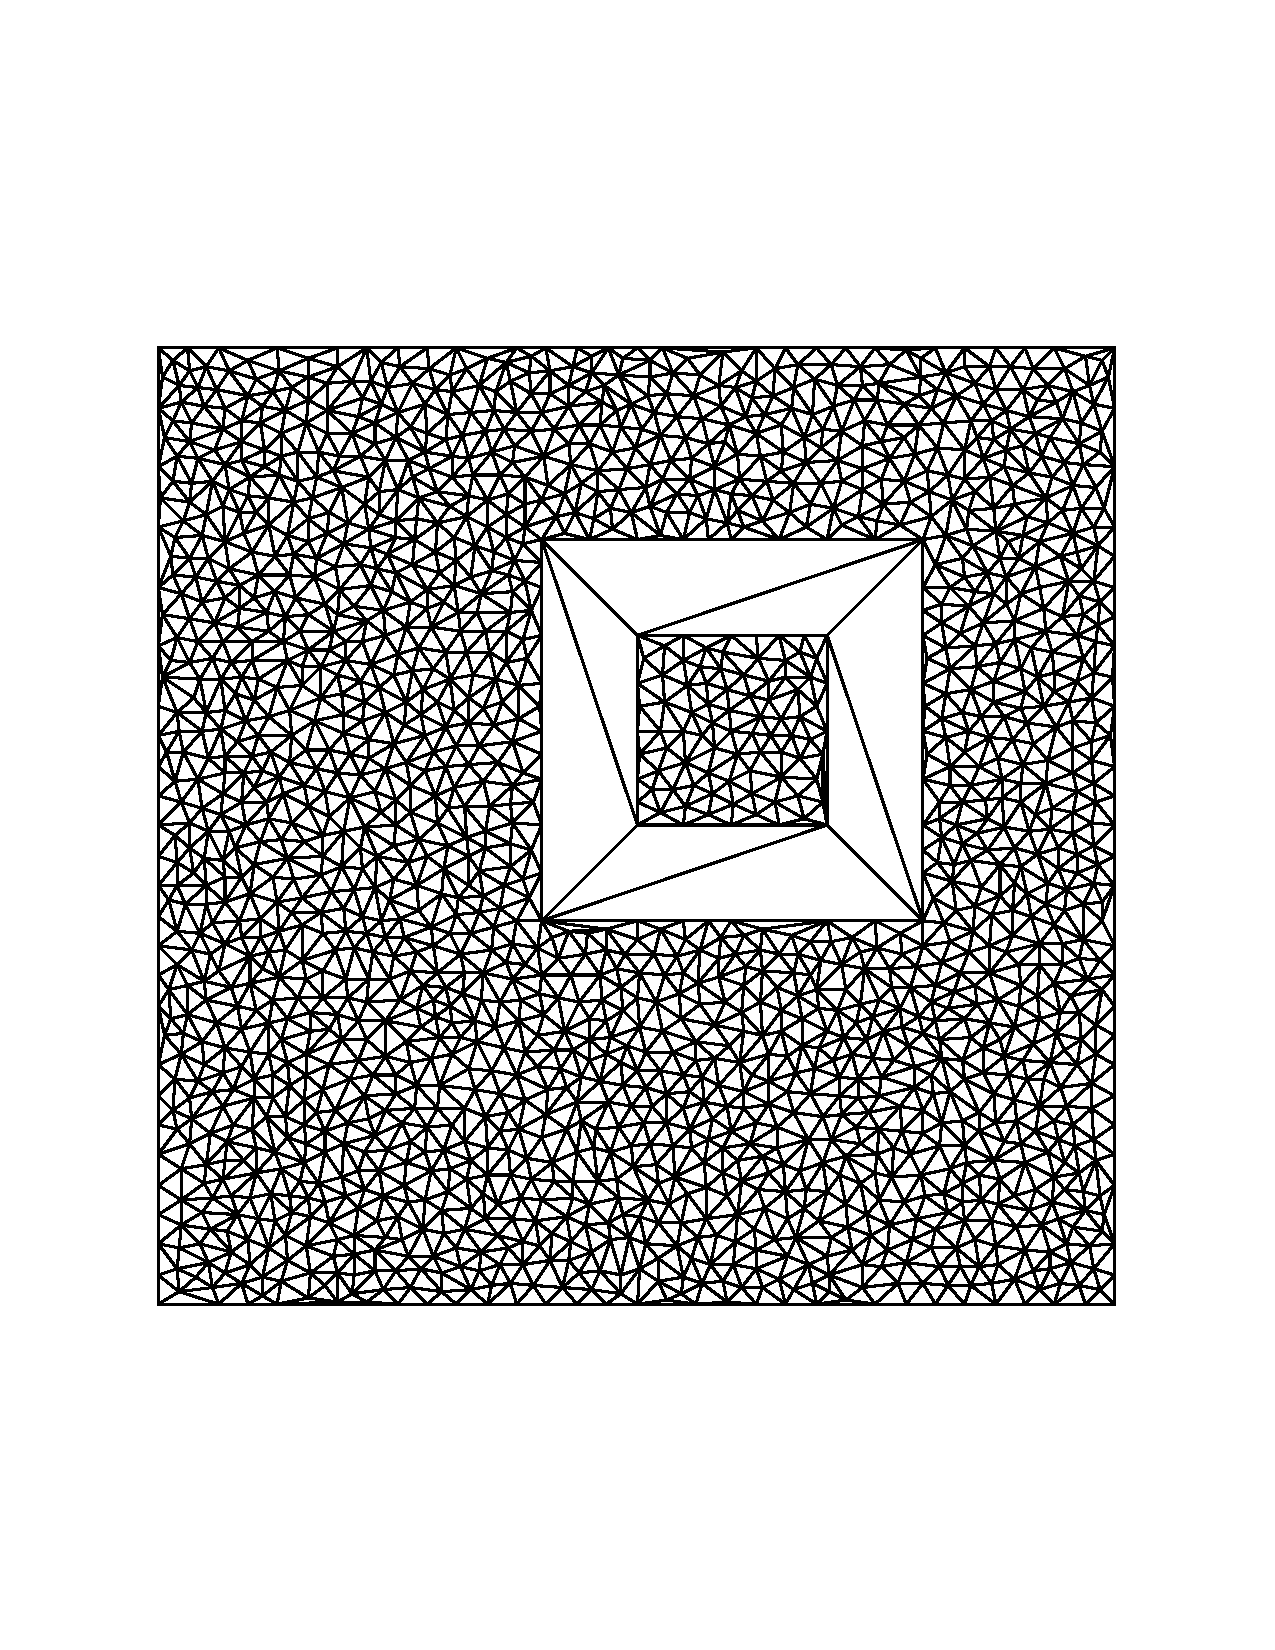
\includegraphics[width=0.5\textwidth]{dziurka.pdf}

\subsubsection{Test z~większym plikiem}
W~ramach tego testu skorzystałem z~pliku poly opisującego literę 'A' złożoną z~kilkudziesięciu trójkątów, który jest dystrybuowany razem z~trianglem.
Test ten zawiera stosunkowo dużo wierzchołków i~pozwolił wykryć problem z~implementacją hasha.
\begin{lstlisting}
./bin/siatkonator -e spec/data/cieciurm/A.1.ele -o test spec/data/square-large.poly
\end{lstlisting}
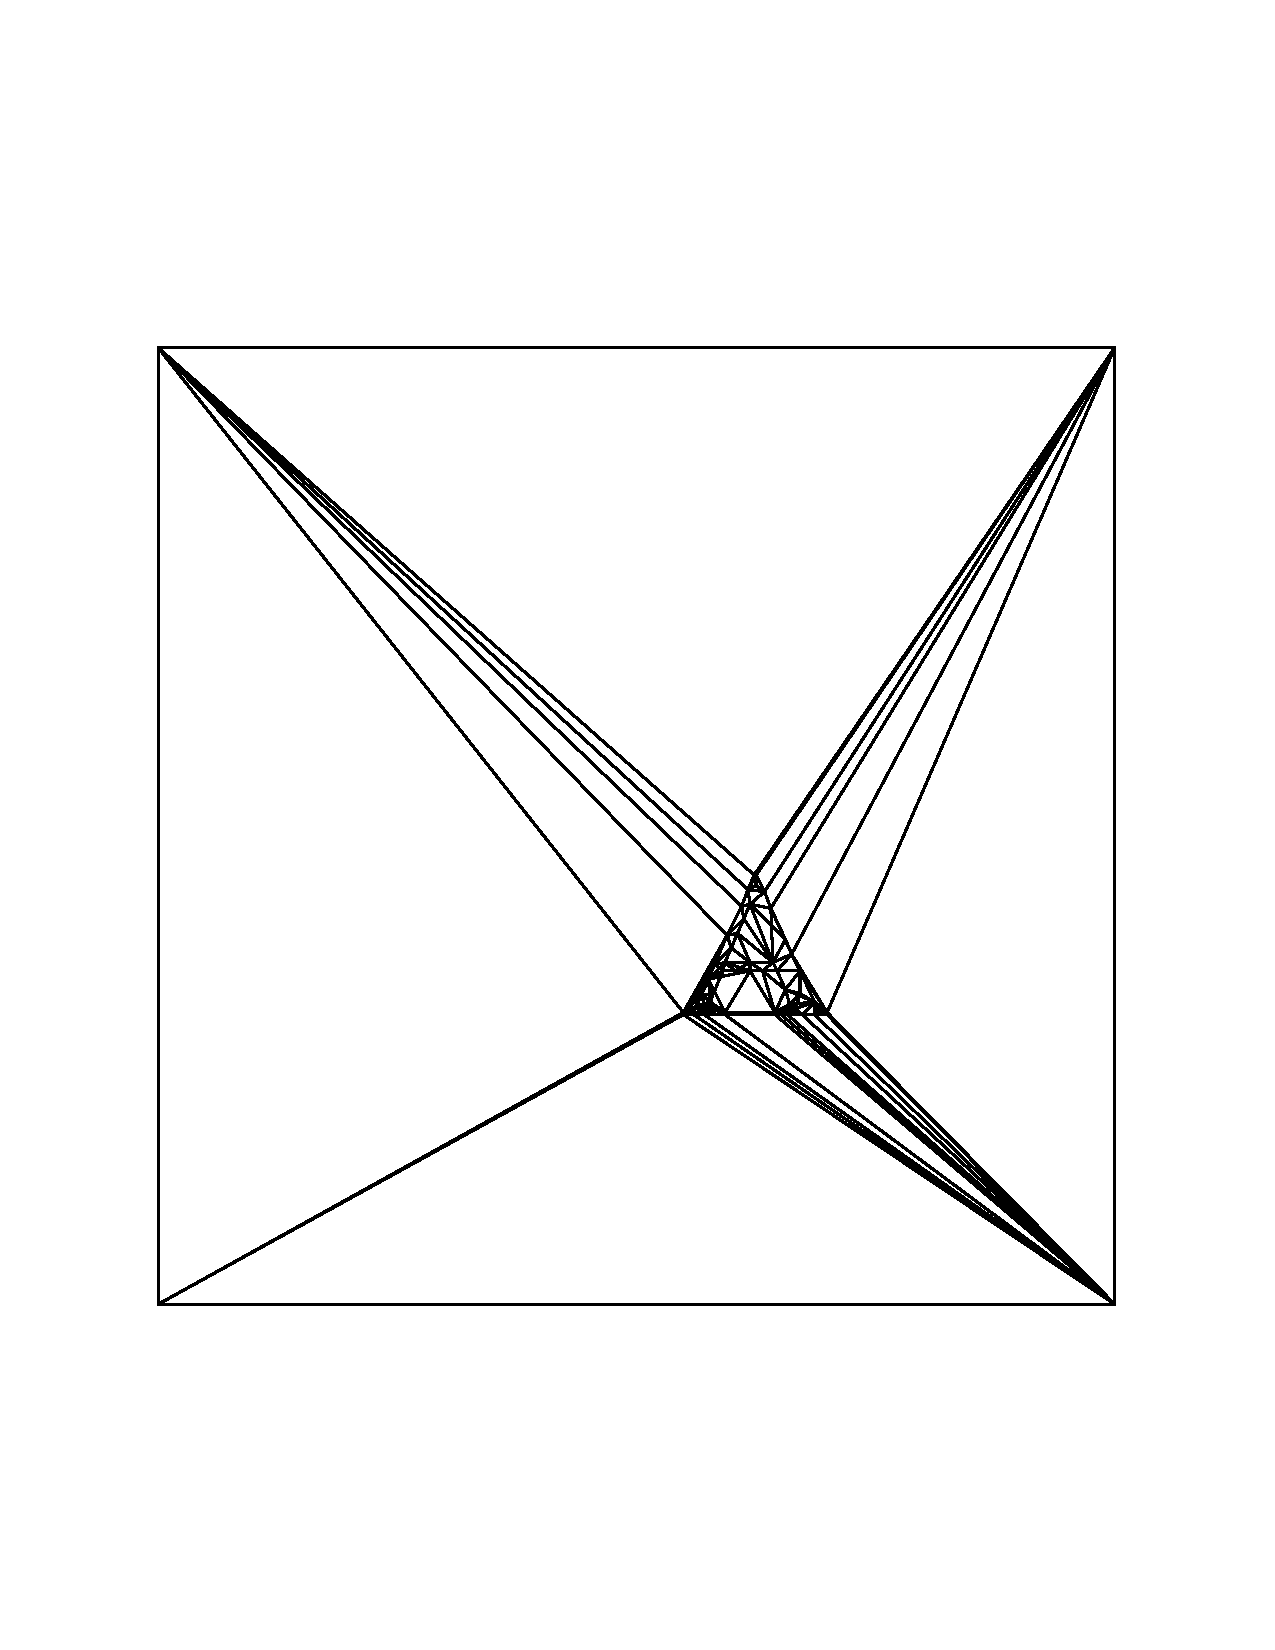
\includegraphics[width=0.5\textwidth]{litera_a.pdf}

\subsubsection{Markery i~atrybuty}
Po włączeniu opcji debug uruchomiłem następujące polecenie, aby sprawdzić że przepisywanie markerów działa zgodnie z~założeniami, a~atrybuty są zachowywane:

\begin{lstlisting}
./bin/siatkonator -e spec/data/attrs+markers/2attr-1mark.ele spec/data/attrs+markers/square-2attr-1mark.poly
\end{lstlisting}

Pliki wejściowe tego testu mają następującą charakterystykę:
\begin{itemize}
  \item plik node zawiera atrybuty od 8080 do 8085 i~markery od 1 do 3
  \item plik poly zawiera atrybuty od 1024 do 1031 i~markery równe 2
\end{itemize}

W~wyniku uruchomienia programu w~trybie \texttt{debug}, uzyskałem następującą informację:

\begin{lstlisting}
marker range change for mesh 0: 1-3 --> 0-2
marker range change for mesh 1: 2-2 --> 3-3
\end{lstlisting}

Należy się więc spodziewać, że w~pliku wyjściowym pliki z~atrybutami 808* będą miały markery zawierające się w~przedziale 0 - 2, natomiast pliki z~atrybutami 10** - równe 3.

Wynik testu to potwierdza:

\begin{lstlisting}
0 -2.000000 -2.000000 1024.000000 1025.000000 3
1 -2.000000 3.000000 1026.000000 1027.000000 3
2 3.000000 3.000000 1028.000000 1029.000000 3
3 3.000000 -2.000000 1030.000000 1031.000000 3
4 1.100000 1.100000 8080.000000 8081.000000 0
5 1.300000 1.100000 8082.000000 8083.000000 1
6 1.100000 1.300000 8084.000000 8085.000000 2
\end{lstlisting}

\subsubsection{Pozostałe}
Udało mi się wygenerować poprawne siatki korzystając z~plików trap i~tri zamieszczonych na wikidydzie. Nie udało mi się znaleźć żadnych plików wejściowych o~poprawnej strukturze, z~których program generowałby nieprawidłowe siatki (z~wyjątkiem kombinacji plików tkaich, że siatka nie zawierała się w~otoczce).

Pliki o~niepoprawnej strukturze powodują nieprawidłowe działąnie programu.

\end{document}
